\documentclass{report}
\usepackage{textcase}
\usepackage{amsmath}
\usepackage{amsfonts}
\usepackage{amssymb}
\usepackage[utf8]{vietnam}
\usepackage{graphicx}
\usepackage{scrextend}
\usepackage[left=3.5cm,right=2cm,top=3.5cm,bottom=3cm]{geometry}
\usepackage{xhfill}
\usepackage{floatrow}
\usepackage{subfigure}
\usepackage{wrapfig}
\usepackage{lipsum}
\usepackage{lettrine}
\usepackage[
    backend=biber,
    style=authoryear,
    natbib=true,
    url=true, 
    doi=true,
    eprint=false
]{biblatex}
\usepackage{hyperref} 
\addbibresource{myref.bib}

\begin{document}
\newcommand{\xfill}[2][1ex]{{%
  \dimen0=#2\advance\dimen0 by #1
  \leaders\hrule height \dimen0 depth -#1\hfill%
}}

%Page 1
\changefontsizes[14pt]{12pt}
\centerline{TỔNG LIÊN ĐOÀN LAO ĐỘNG VIỆT NAM}

\changefontsizes[14pt]{11pt}
\centerline{\textbf{TRƯỜNG ĐẠI HỌC TÔN ĐỨC THẮNG}}
\centerline{\textbf{KHOA CÔNG NGHỆ THÔNG TIN}}

\begin{center}
    \begin{figure}[htp]
    \begin{center}
     
\includegraphics[scale=.2]{logo}
    \end{center}
    \end{figure}
\end{center}

\changefontsizes{16pt}
\centerline{\textbf{BÀI TẬP LỚN: LẬP TRÌNH WEB VÀ ỨNG DỤNG}}
\vspace{1.5cm}
\changefontsizes{24pt}
\centerline{\textbf{TÌM HIỂU NODE JS}}

\vspace{4cm}
\begin{flushright}
\renewcommand{\baselinestretch}{0.05}
\changefontsizes{14pt}
\textit{Người hướng dẫn: }\textbf{G.V Đặng Minh Thắng}
\setlength{\parskip}{0.5em}

\textit{Người thực hiện: }\textbf{Trần Quốc Lĩnh - 51703124}
\setlength{\parskip}{0.5em}

Lớp: \textbf{17050301}
\setlength{\parskip}{0.5em}

Khoá: \textbf{21}
\setlength{\parskip}{0.5em}

\end{flushright}

\vspace{1cm}
\changefontsizes{14pt}
\centerline{\textbf{THÀNH PHỐ HỒ CHÍ MINH, NĂM 2019}}


%Page 2
\newpage
\changefontsizes[14pt]{12pt}
\centerline{TỔNG LIÊN ĐOÀN LAO ĐỘNG VIỆT NAM}

\changefontsizes[14pt]{11pt}
\centerline{\textbf{TRƯỜNG ĐẠI HỌC TÔN ĐỨC THẮNG}}
\centerline{\textbf{KHOA CÔNG NGHỆ THÔNG TIN}}

\begin{center}
    \begin{figure}[htp]
    \begin{center}
     
\includegraphics[scale=.2]{logo}
    \end{center}
    \end{figure}
\end{center}

\changefontsizes{16pt}
\centerline{\textbf{BÀI TẬP LỚN: LẬP TRÌNH WEB VÀ ỨNG DỤNG}}
\vspace{1.5cm}
\changefontsizes{24pt}
\centerline{\textbf{TÌM HIỂU NODE JS}}

\vspace{4cm}
\begin{flushright}
\renewcommand{\baselinestretch}{0.05}
\changefontsizes{14pt}
\textit{Người hướng dẫn: }\textbf{G.V Đặng Minh Thắng}
\setlength{\parskip}{0.5em}

\textit{Người thực hiện: }\textbf{Trần Quốc Lĩnh - 51703124}
\setlength{\parskip}{0.5em}

Lớp: \textbf{17050301}
\setlength{\parskip}{0.5em}

Khoá: \textbf{21}
\setlength{\parskip}{0.5em}

\end{flushright}

\vspace{1cm}
\changefontsizes{14pt}
\centerline{\textbf{THÀNH PHỐ HỒ CHÍ MINH, NĂM 2019}}


% Page 3
\newpage
\changefontsizes{16pt}
\centerline{\textbf{LỜI CẢM ƠN}}

\changefontsizes{13pt}
\bigskip
\setlength{\parindent}{2cm}

Cảm ơn thầy Đặng Minh Thắng đã dạy môn lập trình web và ứng dụng hết sức nhiệt tình và tâm huyết, cảm ơn thầy đã định hướng và tạo cơ sở để em có thể tự tìm hiểu và học thêm về cách lập trình và tổ chức một trang web.

Còn đây là bài tập lớn, một nội dung trong trương trình giảng dạy mà thầy đã giao cho em. Trong quá trình làm bài tập lớn này, em vẫn còn nhiều thiếu sót. Em rất mong nhận được sự đánh giá và chỉ bảo từ thầy!
    
% Page 4
\newpage
\changefontsizes{16pt}
\centerline{\textbf{BÀI TẬP LỚN ĐƯỢC HOÀN THÀNH}}
\centerline{\textbf{TẠI TRƯỜNG ĐẠI HỌC TÔN ĐỨC THẮNG}}
\changefontsizes{13pt}
\vspace{1cm}
\setlength{\parindent}{2cm}
Em xin cam đoan đây là sản phẩm bài tập lớn của riêng em. Các nội dung nghiên cứu, kết quả trong đề tài này là trung thực và chưa công bố dưới bất kỳ hình thức nào trước đây. Những số liệu ,hình ảnh được chính em thu thập từ các nguồn khác nhau có ghi rõ trong phần tài liệu tham khảo.

\setlength{\parindent}{2cm}
Ngoài ra, trong bài tiểu luận còn sử dụng một số nhận xét, đánh giá cũng như số liệu của các tác giả khác, cơ quan tổ chức khác đều có trích dẫn và chú thích nguồn gốc.

\setlength{\parindent}{2cm}
Nếu phát hiện có bất kỳ sự gian lận nào em xin hoàn toàn chịu trách nhiệm về nội dung bài tập lớn của mình. Trường đại học Tôn Đức Thắng không liên quan đến những vi phạm tác quyền, bản quyền do em gây ra trong quá trình thực hiện (nếu có).

\vspace{0.75cm}
\begin{flushright}
\renewcommand{\baselinestretch}{0.05}
\changefontsizes{13pt}
\textit{TP. Hồ Chí Minh, ngày 31 tháng 03 năm 2019}
\end{flushright}

\setlength{\parindent}{12cm}
\textit{Tác giả }\\

\setlength{\parindent}{12cm}
\textit{(Đã ký)}\\

\setlength{\parindent}{11.25cm}
\textit{Trần Quốc Lĩnh}\\



% Page 5
\newpage
\changefontsizes{16pt}
\centerline{\textbf{PHẦN XÁC NHẬN VÀ ĐÁNH GIÁ CỦA GIẢNG VIÊN}}
\bigskip
\changefontsizes{13pt}
\setlength{\parindent}{2.2cm}
Phần xác nhận của GV hướng dẫn

\vspace{0.8cm}
\setlength{\parindent}{1cm}
\ \xfill{1pt} \

\bigskip
\ \xfill{1pt} \

\bigskip
\ \xfill{1pt} \

\bigskip
\ \xfill{1pt} \

\bigskip
\ \xfill{1pt} \

\bigskip
\ \xfill{1pt} \

\changefontsizes{12pt}
\setlength{\parindent}{8cm}
Tp. Hồ Chí Minh, ngày 31 tháng 03 năm 2019

\setlength{\parindent}{11cm}
\textit{(kí và ghi họ tên)}

\changefontsizes{13pt}
\vspace{2.5cm}
\setlength{\parindent}{2.2cm}
Phần đánh giá của GV chấm bài

\vspace{0.8cm}
\setlength{\parindent}{1cm}
\ \xfill{1pt} \

\bigskip
\ \xfill{1pt} \

\bigskip
\ \xfill{1pt} \

\bigskip
\ \xfill{1pt} \

\bigskip
\ \xfill{1pt} \

\bigskip
\ \xfill{1pt} \

\changefontsizes{12pt}
\setlength{\parindent}{8cm}
Tp. Hồ Chí Minh, ngày 31 tháng 03 năm 2019

\setlength{\parindent}{11cm}
\textit{(kí và ghi họ tên)}

% Page 6
\newpage
\changefontsizes{16pt}
\centerline{\textbf{TÓM TẮT}}\

\changefontsizes{13pt}
\setlength{\parindent}{2cm}
Internet đã xuất hiện hơn một thập kỷ qua, và sự phổ biến của nó đã được lan rộng trên toàn cầu. Nên là hầu như trong mỗi chúng ta ai ai cũng biết một trang web trông thế nào, có nhiều loại ra sao. Nhưng không nhiều người biết đến cách một trang web được tạo ra và vận hành như thế nào. Và trong bài tập lớn này, em xin trình bài một nội dung, một phương thức dùng để quản lí và vận hành server của web. Node JS

Gồm có các nội dung chính:

\setlength{\parindent}{3cm}
- Tổng quan về Node JS

- Thiết kế một web chat đơn giản bằng Node JS

%Page 7
\newpage
\changefontsizes{16pt}
\centerline{\textbf{MỤC LỤC}}\

\vspace{1.2cm}
\changefontsizes{14pt}
\setlength{\parindent}{0cm}
LỜI CẢM ƠN\dotfill\ 3

\smallskip
CAM KẾT\dotfill\ 4

\smallskip
ĐÁNH GIÁ CỦA GIÁO VIÊN\dotfill\ 5

\smallskip
TÓM TẮT\dotfill\ 6

\smallskip
MỤC LỤC\dotfill\ 7

\smallskip
DANH MỤC CHÚ THÍCH CÁC THUẬT NGỮ VÀ HÌNH ẢNH\dotfill\ 8

\smallskip
TỔNG QUAN VỀ NODE JS\dotfill\ 9

\setlength{\parindent}{0.5cm}
1. Node JS là gì?\dotfill\ 9

2. Đặc điểm của Node JS?\dotfill\ 10

3. Cơ chế hoạt động\dotfill\ 10

4. Ứng dụng của Node JS\dotfill\ 11

5. Ưu điểm và nhược điểm\dotfill\ 11

\setlength{\parindent}{0cm}
\smallskip
THIẾT KẾ MỘT WEB CHAT ĐƠN GIẢN BẰNG NODE JS\dotfill\ 12

\setlength{\parindent}{0.5cm}
1. Cách cài đặt và chạy demo\dotfill\ 12

2. Mô tả code\dotfill\ 18

\setlength{\parindent}{0cm}
\smallskip
TÀI LIỆU THAM KHẢO\dotfill\ 21

%Page 8
\newpage
\changefontsizes{16pt}
\centerline{\textbf{DANH MỤC CHÚ THÍCH CÁC THUẬT NGỮ}}
\centerline{\textbf{VÀ HÌNH ẢNH}}

\vspace{1cm}
\changefontsizes{14pt}
\textbf{Thuật ngữ}

\changefontsizes{13pt}
\bigskip
\textbf{Heap} : Là vùng nhớ được dùng để chứa kết quả tạm phục vụ cho việc thực thi các hàm trong stack. Heap càng lớn thì khả năng tính toán càng cao.

\smallskip
\textbf{Stack} : Là một kiểu hàng đợi first in last out - vào trước ra sau.

\smallskip
\textbf{Js runtime engine} : Là khu thực thi câu lệnh js gồm Heap và stack.

\smallskip
\textbf{Web APIs} : Là nơi chức các tác vụ được cung cấp bởi trình duyệt.

\smallskip
\textbf{Callback queue} : Là hàng đợi công việc kiểu first in first out - vào trước ra trước.

\smallskip
\textbf{Event Loop} :  Đọc Stack và Event Queue. Nếu nhận thấy Stack rỗng nó sẽ nhặt Event đầu tiên trong Event Queue và handler (callback hoặc listener) gắn với Event đó và đẩy vào Stack. Đặc điểm của việc thực thi hàm trong JS là sẽ chỉ dừng lại khi hàm return hoặc throw exception. Có nghĩa là trong khi hàm đang chạy thì sẽ không có một hàm khác được chạy, dữ liệu tạm của hàm cũng sẽ không bị thay đổi bởi một hàm khác hay cũng không bị dừng lại cho đến khi hoàn thành.

\changefontsizes{14pt}
\bigskip
\textbf{Hình ảnh}

\bigskip
\changefontsizes{13pt}
Hình 1: Các định nghĩa của Node JS

Hình 2: Cơ chế hoạt động

Hình 3: Download Node JS

Hình 4: Cách cài đặt - Chọn next

Hình 5: Cách cài đặt - Tick vào ô I accept và chọn next

Hình 6: Cách cài đặt - Chọn thư mục để cài rồi chọn next

Hình 7: Cách cài đặt - Chọn next

Hình 8: Cách cài đặt - Chọn next

Hình 9: Cách cài đặt - Đợi cho đến khi việc cài đặt hoàn tất

Hình 10: Cách cài đặt - Chọn finish

Hình 11: Cài đặt module cho Node JS để chạy realtime

Hình 12: Lệnh thực thi trên cmd

Hình 13: Trên cửa sổ trình duyệt

Hình 14: Demo chat real time

Hình 15: Khởi tạo biến và import module cần thiết

Hình 16: Load một trang html từ file

Hình 17: Tạo một server lắng nghe trên cổng 8000

Hình 18: Tạo biến kết nối với server trên cổng 8000

Hình 19: Client giao tiếp với server

Hình 20: Server handle các sự kiện client gửi tới

%Page ??
\newpage
\changefontsizes{16pt}
\centerline{\textbf{TỔNG QUAN VỀ NODE JS}}

\bigskip
\changefontsizes{14pt}
1. Node JS là gì?

\smallskip
\setlength{\parindent}{1cm}
Node js là một mã nguồn mở, một môi trường, một hệ thống phần mềm được thiết kế để viết các ứng dụng internet có khả năng mở rộng, đặc biệt là máy chủ web. Là một nền tảng chạy trên môi trường V8 JavaScript runtime - một trình thông dịch JavaScript cực nhanh, theo thời gian thực chạy trên trình duyệt Chrome.

Phần Core bên dưới của Node js được viết hầu hết bằng C++ nên cho tốc độ xử lý và hiệu năng khá cao.

Node js chứa một thư viện built-in cho phép các ứng dụng hoạt động như một Webserver mà không cần phần mềm như Nginx, Apache HTTP Server hoặc IIS.

Mọi hàm trong Node js là không đồng bộ (asynchronous). Do đó, các tác vụ đều được xử lý và thực thi ở chế độ nền (background processing)

Node.js được tạo bởi Ryan Dahl từ năm 2009, và phát triển dưới sự bảo trợ của Joyent.

\begin{center}
    \begin{figure}[htp]
    \begin{center}
     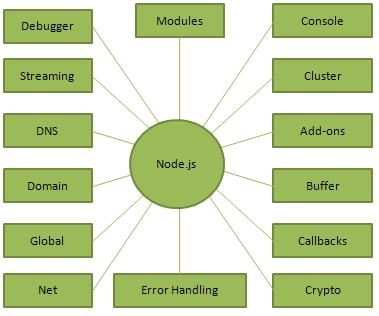
\includegraphics[scale=1]{nodejs_concepts.jpg}
    \end{center}
    \caption{Các định nghĩa của Node JS}
    \label{refhinh1}
    \end{figure}
\end{center}

\setlength{\parindent}{0cm}
2. Đặc điểm của Node JS

\smallskip
\setlength{\parindent}{1cm}
- Node JS là không phải là một ngôn ngữ mà nó chỉ là môi trường để chạy javascript phía server. 

- Node JS nó có tất cả các tính chất của javascript.

- Node JS xử lý bất đồng bộ.

- Node JS chạy đơn luồng. Tức là Node JS chạy trên 1 CPU core duy nhất.

- Là ngôn ngữ hướng sự kiện.

\bigskip
\setlength{\parindent}{0cm}
3. Cơ chế hoạt động
\begin{center}
    \begin{figure}[htp]
    \begin{center}
     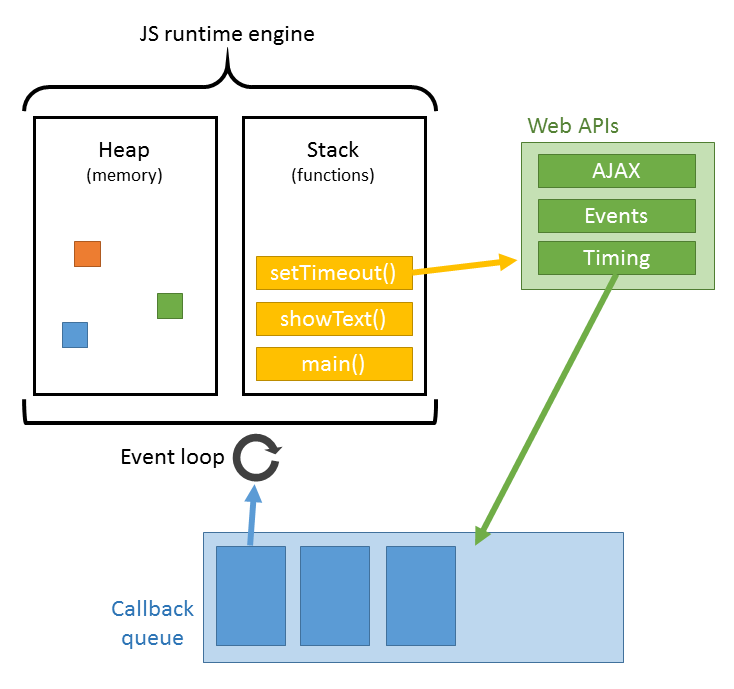
\includegraphics[scale=.3]{1.png}
    \end{center}
    \caption{Cơ chế hoạt động}
    \label{refhinh1}
    \end{figure}
\end{center}

\smallskip
\setlength{\parindent}{1cm}
B1: Đầu tiên các câu lệnh được chạy lần lượt từ trên xuống dưới và đưa vào hàng đợi queue.

B2: Vì lúc này stack vẫn trống nên event loop sẽ lấy một tác vụ ở trong queue bỏ vào stack. 

B3: Sau khi xử lý xong thì tác vụ đó sẽ được lấy ra khỏi stack, và cho tác vụ tiếp theo vào. Nếu ta thấy có một hàm nào đó trong web AIPs dùng để tính toán thời gian, nó sẽ được đưa vào Web APIs để đợi.

B4: Thực hiện các tác vụ còn lại tương tự như trên, cho đến khi hàng đợi rỗng, thì tác vụ đang đợi ở web APIs sẽ được đưa vào stack để thực hiện.


\bigskip
\setlength{\parindent}{0cm}
4. Ứng dụng của Node JS

\smallskip
\setlength{\parindent}{1cm}
- Websocket server: Chat Online, Game online...

- Fast File Upload Client: Các chương trình upload file tốc độ cao.

- Ad server: Máy chủ quảng cáo.

- Cloud services: Các dịch vụ đám mây.

- RESTful API: Dùng cho các ứng dụng thông qua API.

- Any Real-time Data Application: Các ứng dụng yêu cầu tốc độ thời gian thực.\\

\bigskip
\setlength{\parindent}{0cm}
5. Ưu điểm và nhược điểm

\smallskip
* Ưu điểm:

\setlength{\parindent}{1cm}
- Xử lý được nhiều yêu cầu chỉ bằng đơn luồng (single thread). Giúp hệ thống đỡ tốn tài nguyên và tối ưu tốc độ thực thi, giảm độ trễ.

- Có cơ chế event-driven, và mô hình kết hợp với Javascript đáp ứng tốt cho các dịch vụ web.

- Có khả năng sử lý được rất nhiều request mà không cần tải lại trang và khả năng phản hồi nhanh.

- Node JS xây dựng các Proxy phân vùng các luồng dữ liệu để đảm bảo tối đa hoạt động cho các luồng dữ liệu khác.

- Rất hiệu quả khi xây dựng những ứng dụng thời gian thực.

\setlength{\parindent}{0cm}
\smallskip
* Nhược điểm:

\setlength{\parindent}{1cm}
- Khi cần sử dụng những ứng dụng tốn tài nguyên CPU như encoding cho video, convert file,... hay tương tự làm cho chương trình nặng nề tốn tài nguyên. Hiệu suất hoạt động kém.

- Node JS còn sơ khai và nhiều mặt vẫn chưa đáp ứng tốt.


\newpage
\changefontsizes{16pt}
\centerline{\textbf{THIẾT KẾ WEB CHAT ĐƠN GIẢN BẰNG NODE JS}}

\bigskip
\changefontsizes{14pt}
\setlength{\parindent}{0cm}
1. Cách cài đặt và chạy demo.

\setlength{\parindent}{1cm}
Để sử dụng được thì trước hết ta phải cài đặt Node JS vào máy. Truy cập trang web dưới đây theo đường link \url{https://nodejs.org/en/download/} để tiến hành download và cài đặt. Ở đây chọn mục Windows Installer(.msi) 64-bit.

\begin{center}
    \begin{figure}[htp]
    \begin{center}
     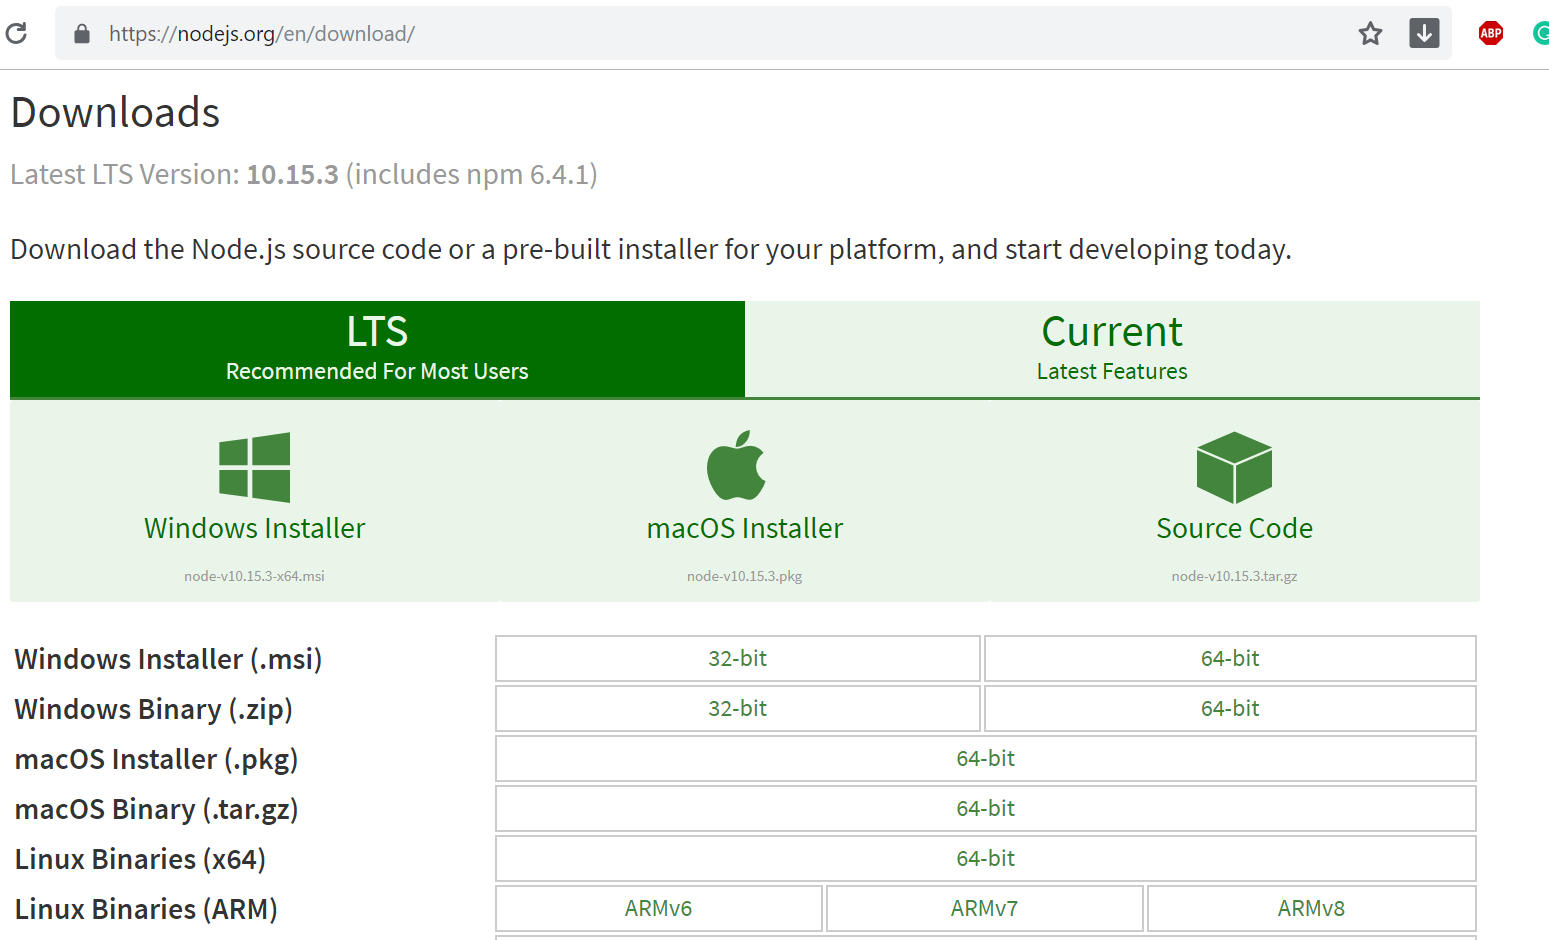
\includegraphics[scale=.55]{download.png}
    \end{center}
    \caption{Download Node JS}
    \label{refhinh1}
    \end{figure}
\end{center}

Sau khi tải xong, chúng ta mở file đó để bắt đầu cài lên máy. Lần lượt theo cái bước sau.


\begin{center}
    \begin{figure}[htp]
    \begin{center}
     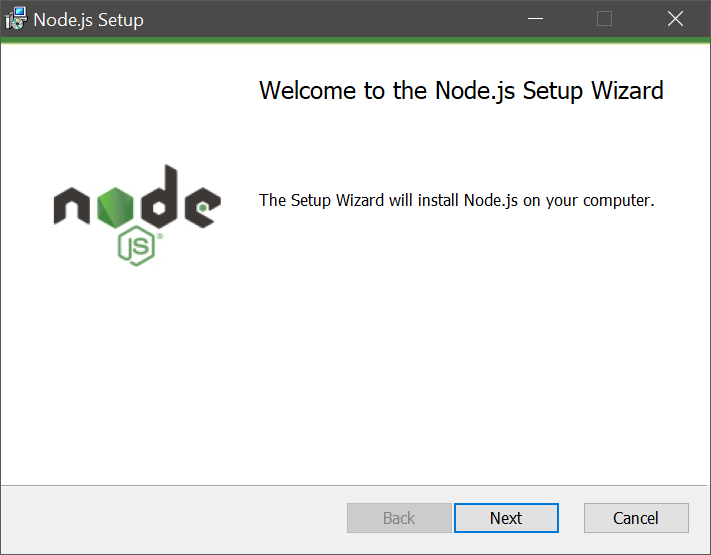
\includegraphics[scale=0.9]{install1.png}
    \end{center}
    \caption{Cách cài đặt - Chọn next}
    \label{refhinh1}
    \end{figure}
\end{center}

\begin{center}
    \begin{figure}[htp]
    \begin{center}
     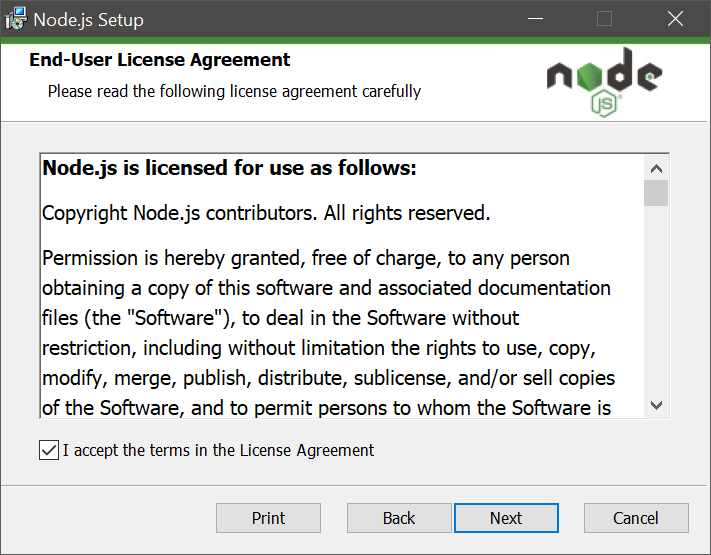
\includegraphics[scale=0.9]{install2.png}
    \end{center}
    \caption{Cách cài đặt - Tick vào ô I accept và chọn next}
    \label{refhinh1}
    \end{figure}
\end{center}

\begin{center}
    \begin{figure}[htp]
    \begin{center}
     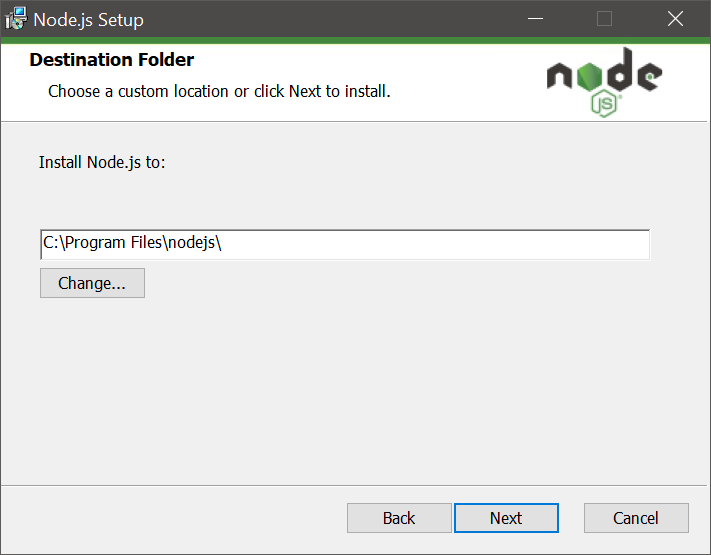
\includegraphics[scale=0.9]{install3.png}
    \end{center}
    \caption{Cách cài đặt - Chọn thư mục để cài rồi chọn next}
    \label{refhinh1}
    \end{figure}
\end{center}

\begin{center}
    \begin{figure}[htp]
    \begin{center}
     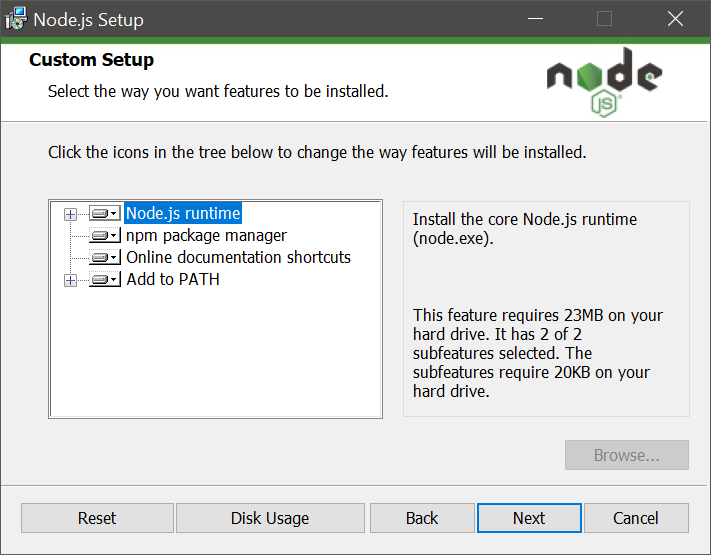
\includegraphics[scale=0.9]{install4.png}
    \end{center}
    \caption{Cách cài đặt - Chọn next}
    \label{refhinh1}
    \end{figure}
\end{center}

\begin{center}
    \begin{figure}[htp]
    \begin{center}
     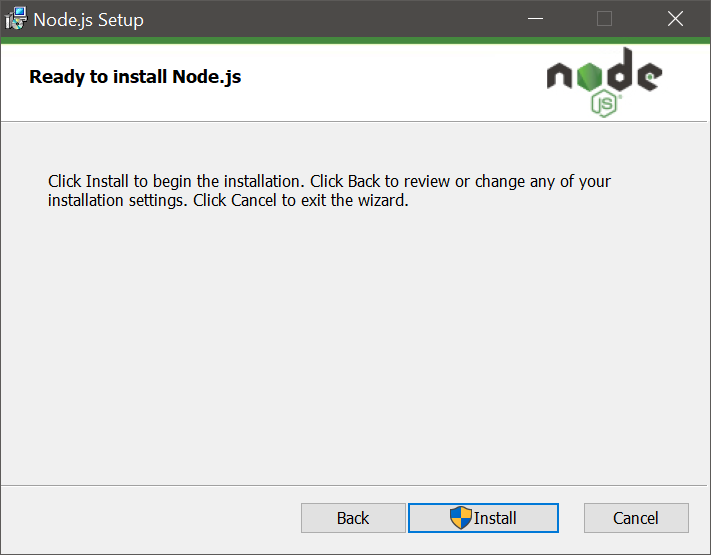
\includegraphics[scale=0.9]{install5.png}
    \end{center}
    \caption{Cách cài đặt - Chọn next}
    \label{refhinh1}
    \end{figure}
\end{center}

\begin{center}
    \begin{figure}[htp]
    \begin{center}
     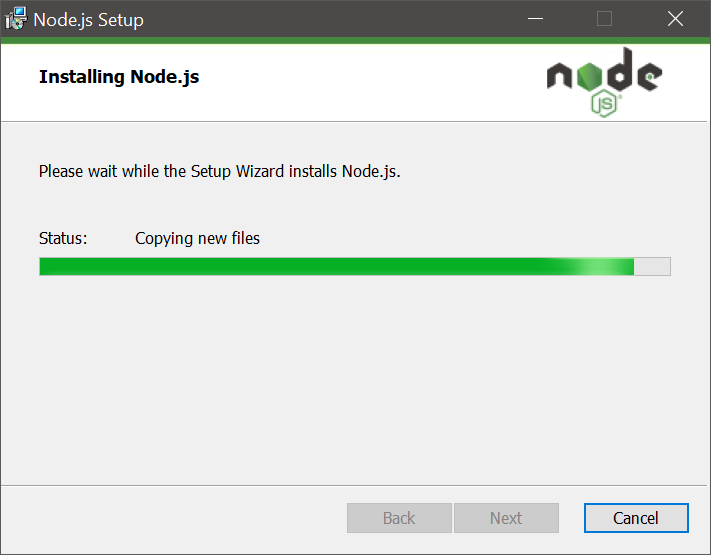
\includegraphics[scale=0.9]{install6.png}
    \end{center}
    \caption{Cách cài đặt - Đợi cho đến khi việc cài đặt hoàn tất}
    \label{refhinh1}
    \end{figure}
\end{center}

\begin{center}
    \begin{figure}[htp]
    \begin{center}
     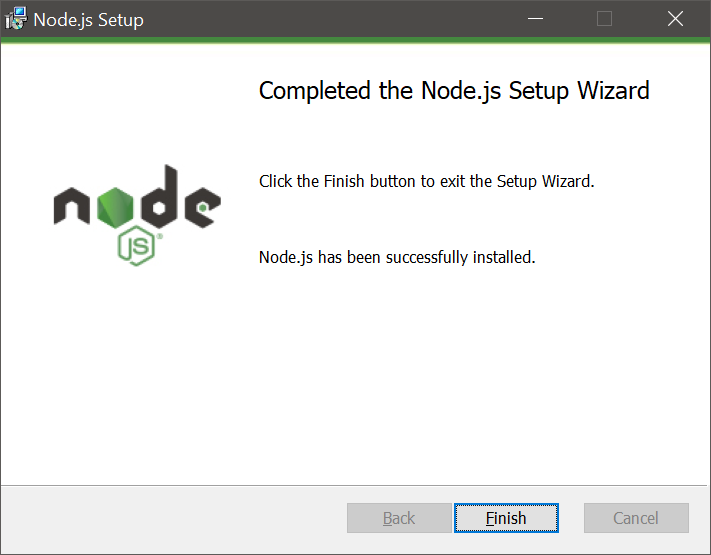
\includegraphics[scale=0.9]{install7.png}
    \end{center}
    \caption{Cách cài đặt - Chọn finish}
    \label{refhinh1}
    \end{figure}
\end{center}

\smallskip

Vậy là việc cài đặt node js đã hoàn tất, kế đến chúng ta cần cài đặt thêm một số module cần thiết để chạy được code demo. Mở cửa sổ cmd lên và dẫn tới thư mục chứa code demo và chạy câu lệnh sau

"npm install socket.io" --save (Đây là đoạn lệnh cài đặt module socket.io hỗ trợ cho việc chạy realtime)

\begin{center}
    \begin{figure}[htp]
    \begin{center}
     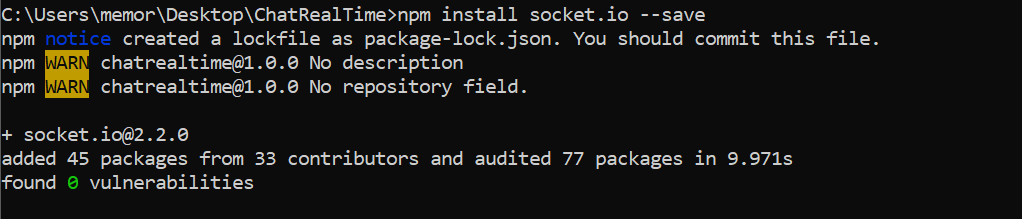
\includegraphics[scale=0.8]{module.png}
    \end{center}
    \caption{Cài đặt module cho Node JS để chạy realtime}
    \label{refhinh1}
    \end{figure}
\end{center}


Bây giờ ta tiến hành chạy code demo, dùng lệnh "node server.js" trên cmd để chạy và mở trang 2 tab của trình duyệt và truy cập đường dẫn \url{http://localhost:8000/} để quan sát việc chạy realtime của node JS thông qua một ứng dụng chat đơn giản.

\begin{center}
    \begin{figure}[htp]
    \begin{center}
     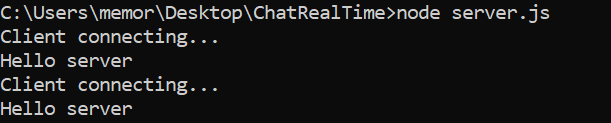
\includegraphics[scale=1.2]{run.png}
    \end{center}
    \caption{Lệnh thực thi trên cmd}
    \label{refhinh1}
    \end{figure}
\end{center}

\begin{center}
    \begin{figure}[htp]
    \begin{center}
     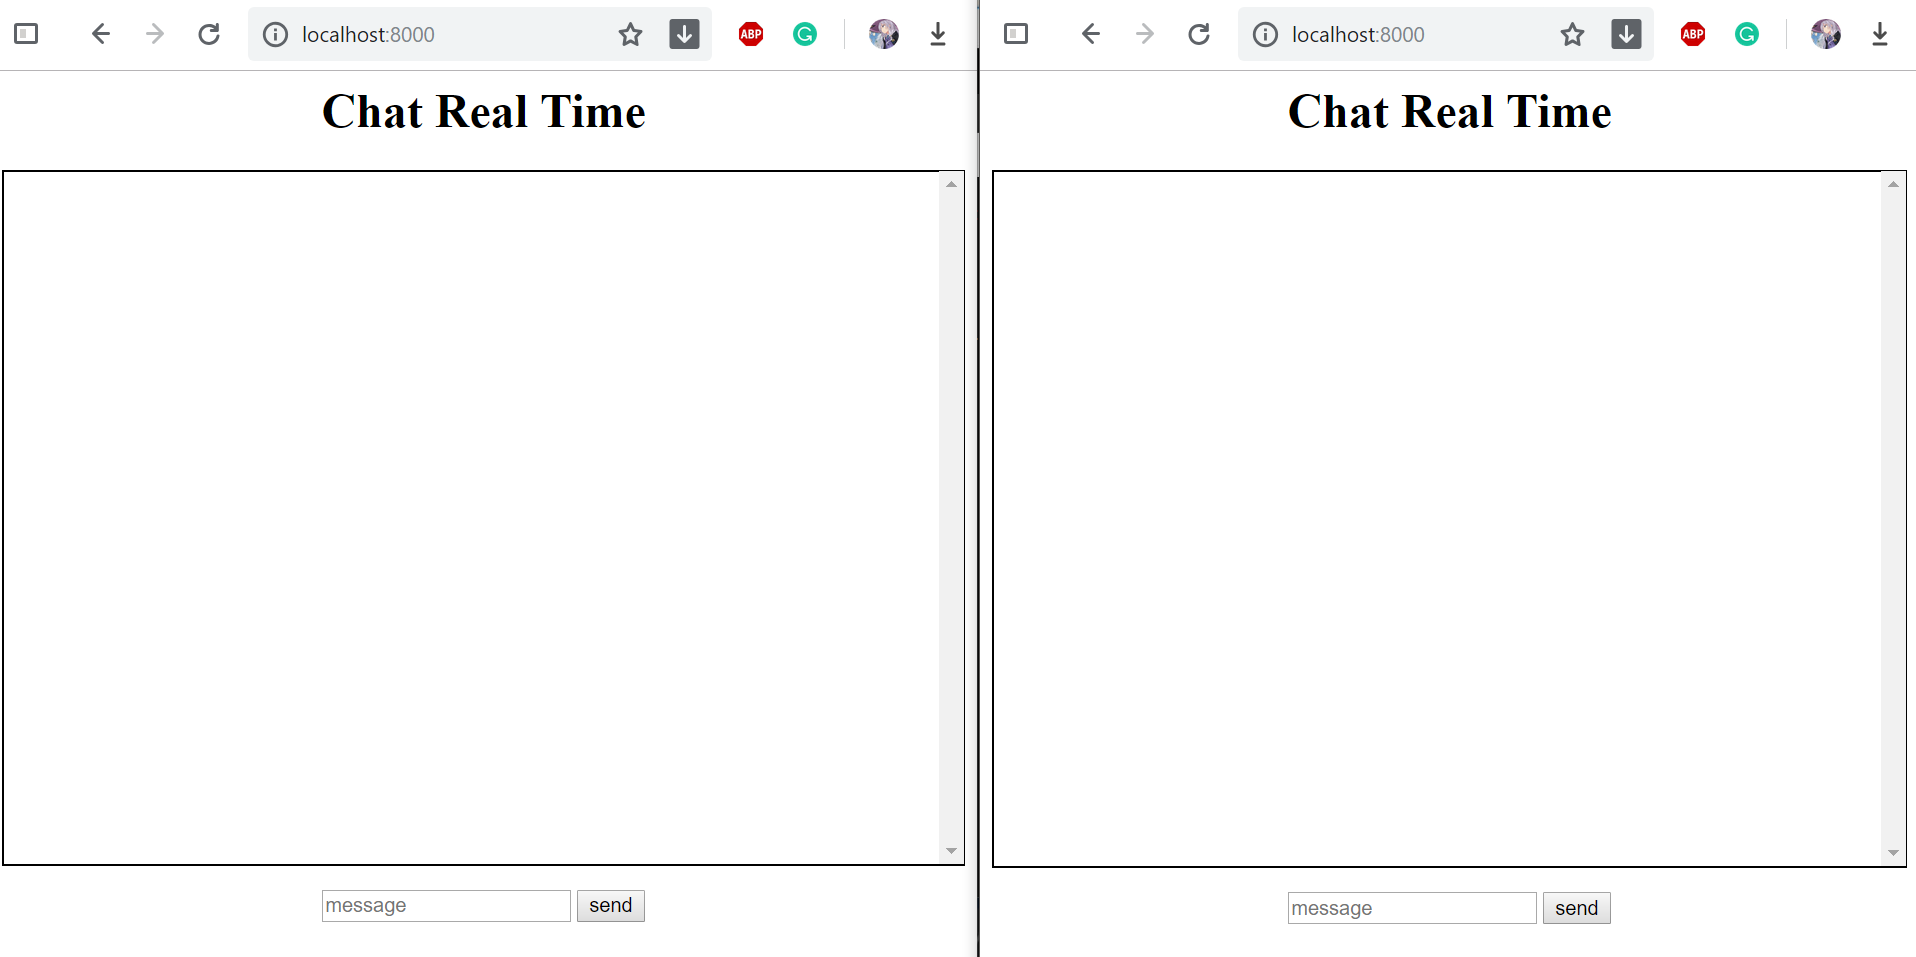
\includegraphics[scale=0.4]{chat.png}
    \end{center}
    \caption{Trên cửa sổ trình duyệt}
    \label{refhinh1}
    \end{figure}
\end{center}

Người dùng tự nhập một số đoạn văn bản ngắn vào ô message rồi click vào nút send trên cả hai tab để quan sát tính realtime mà node js mang lại, dưới đây là ví dụ mẫu.

\begin{center}
    \begin{figure}[htp]
    \begin{center}
     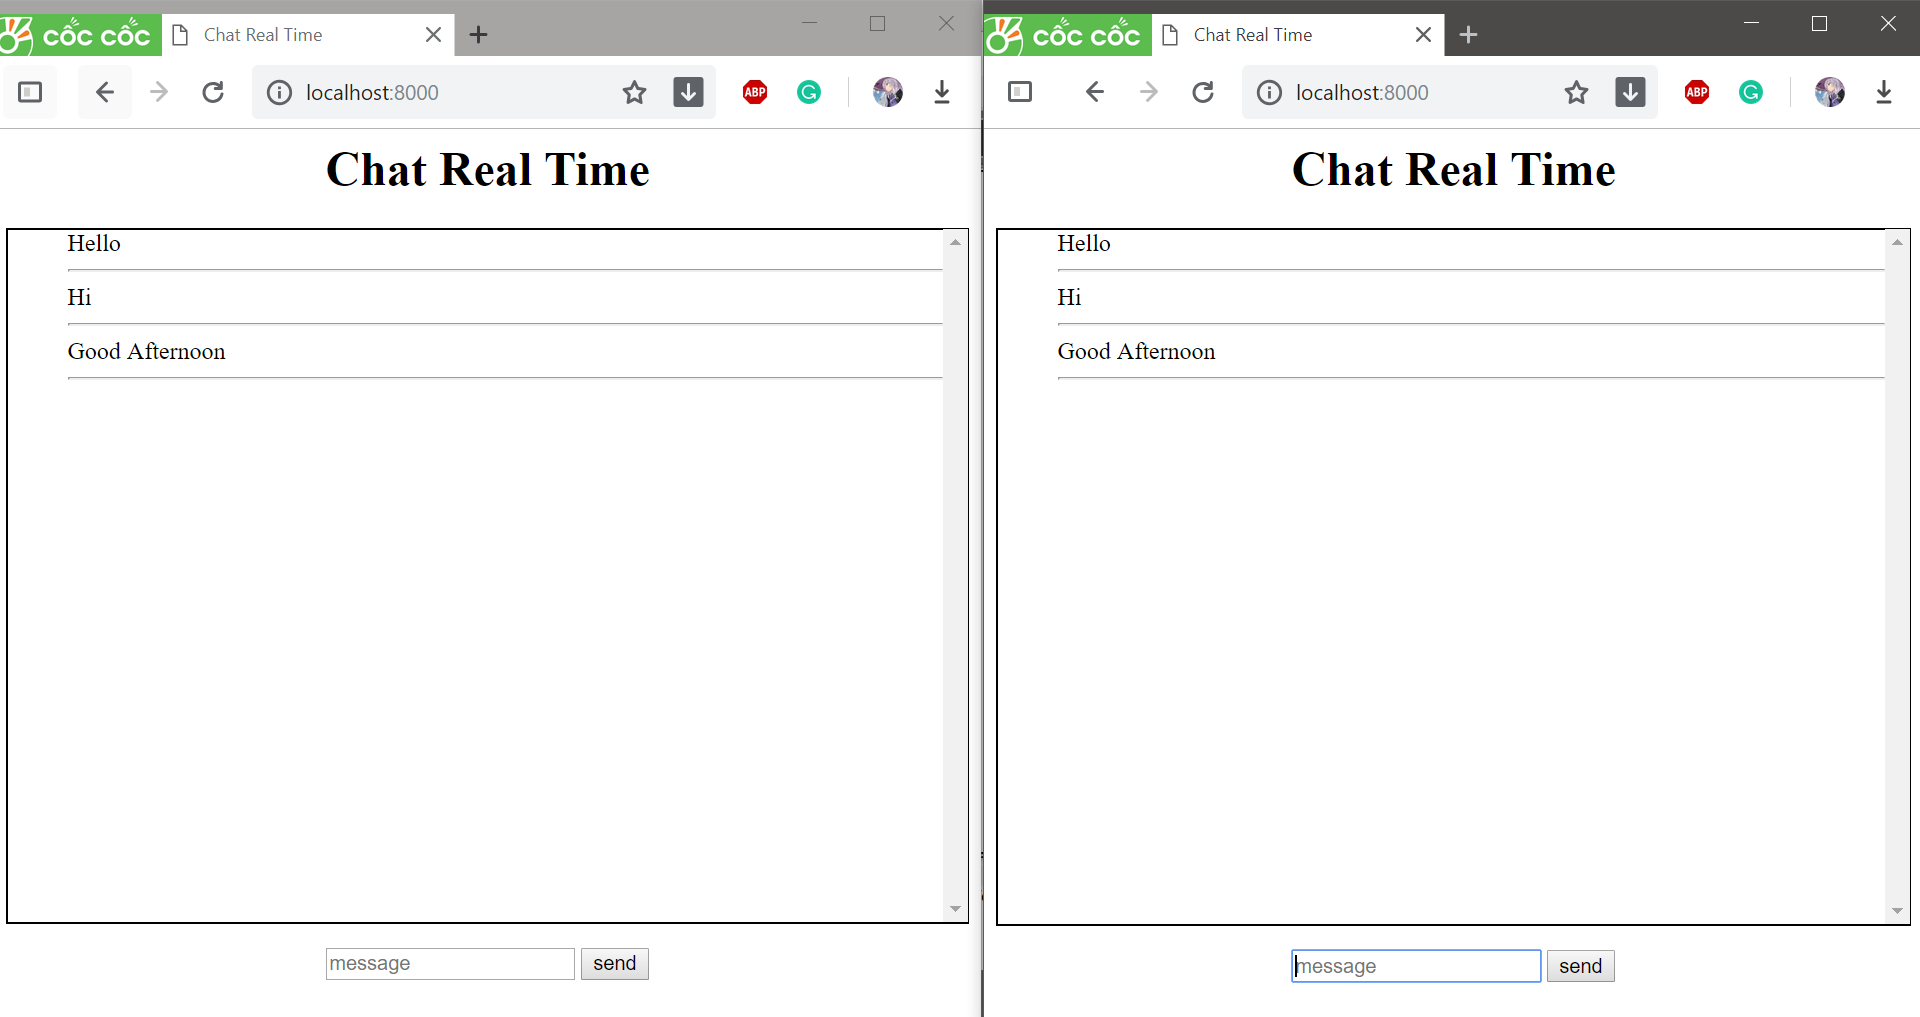
\includegraphics[scale=0.4]{chat2.png}
    \end{center}
    \caption{Demo chat real time}
    \label{refhinh1}
    \end{figure}
\end{center}

\newpage

\newpage

\newpage
\bigskip
\changefontsizes{14pt}
\setlength{\parindent}{0cm}
2. Mô tả code.

\setlength{\parindent}{1cm}
Trong phần code demo gồm có:

- 1 file server.js

- 1 file package.json lưu trữ các thông tin.

- 1 thư mục public chứa: 1 file index.html, 1 file client.js, 1 file style.css.

\setlength{\parindent}{0cm}
*Đối với server

a)Khởi tạo

\begin{center}
    \begin{figure}[htp]
    \begin{center}
     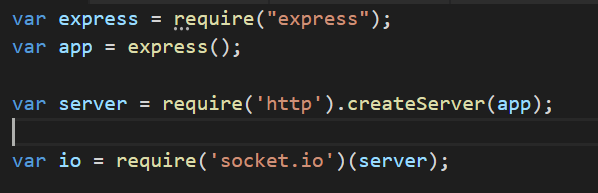
\includegraphics[scale=1.2]{initi.png}
    \end{center}
    \caption{Khởi tạo biến và import module cần thiết}
    \label{refhinh1}
    \end{figure}
\end{center}

b)Load trang web html

\begin{center}
    \begin{figure}[htp]
    \begin{center}
     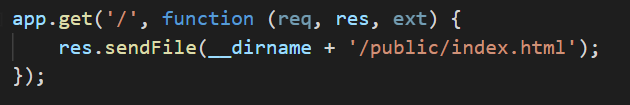
\includegraphics[scale=1.2]{load.png}
    \end{center}
    \caption{Load một trang html từ file}
    \label{refhinh1}
    \end{figure}
\end{center}

c)Tạo một server

\begin{center}
    \begin{figure}[htp]
    \begin{center}
     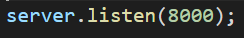
\includegraphics[scale=1.2]{server.png}
    \end{center}
    \caption{Tạo một server lắng nghe trên cổng 8000}
    \label{refhinh1}
    \end{figure}
\end{center}

\bigskip
*Đối với client

a)Khởi tạo
\begin{center}
    \begin{figure}[htp]
    \begin{center}
     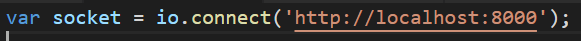
\includegraphics[scale=1.2]{client.png}
    \end{center}
    \caption{Tạo biến kết nối với server trên cổng 8000}
    \label{refhinh1}
    \end{figure}
\end{center}

*Giao tiếp giữa server và client

a) Phía client

- Client handle sự kiện connect và gửi một sự kiện join lên server.

- Client handle sự kiện thread và thêm một thông tin vào trang html.

- Client handle sự kiện submit của form và gửi dữ liệu về cho server qua sự kiện message.


\begin{center}
    \begin{figure}[htp]
    \begin{center}
     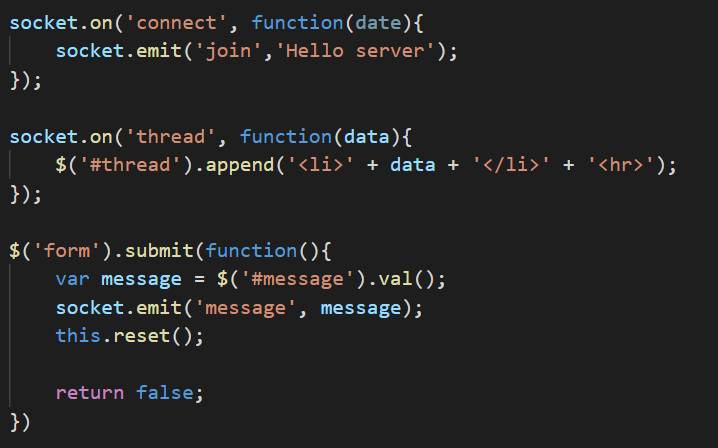
\includegraphics[scale=1]{talk1.png}
    \end{center}
    \caption{Client giao tiếp với server}
    \label{refhinh1}
    \end{figure}
\end{center}

\newpage
b) Phía server

- Server handle sự kiện connect.

- Server handle sự kiện join.

- Server handle sự kiện message và gửi broadcase cho tất cả biết là có một sự kiện thread vừa được tạo ra kèm theo data.

\begin{center}
    \begin{figure}[htp]
    \begin{center}
     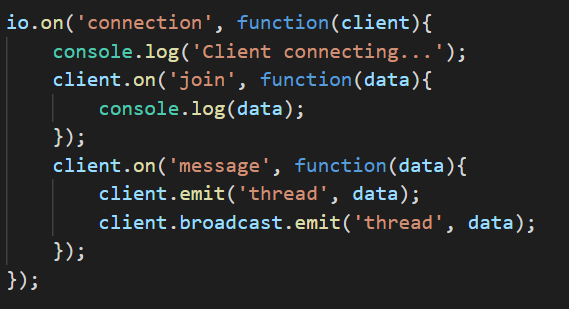
\includegraphics[scale=1]{talk2.png}
    \end{center}
    \caption{Server handle các sự kiện client gửi tới}
    \label{refhinh1}
    \end{figure}
\end{center}

\newpage


\newpage
%Page ?? + 1
\newpage
\changefontsizes{16pt}
\centerline{\textbf{TÀI LIỆU THAM KHẢO}}

\vspace{1.2cm}
\changefontsizes{14pt}
\textbf{Tiếng Việt}

https://vi.wikipedia.org/wiki/Node.js

https://viblo.asia/p/tim-hieu-ve-node-js-co-ban-ojaqG0dGEKwZ

https://techtalk.vn/mot-cai-nhin-tong-quan-nhat-ve-nodejs.html

https://techblog.vn/tim-hieu-ve-node-js-co-ban

\vspace{3cm}
\textbf{Tiếng Anh}

https://nodejs.org/en/docs/


\end{document}